\documentclass[a4paper,10pt,twoside,draft]{article}

\usepackage[english]{babel}
\usepackage{amssymb}
\usepackage{fancyhdr}
\usepackage{graphicx}
\usepackage[ocgcolorlinks]{hyperref}

\pagestyle{fancy}
\fancyhead{}
\fancyfoot{}
\fancyhead[RE,LO]{de Kok \& Methenitis}
\fancyhead[RO,LE]{Week 2}
\fancyfoot[RE]{\thepage$\quad \square$}
\fancyfoot[LO]{$\square \quad$\thepage}

\title{Report for Week 2\\\normalsize Sift and its applications}

\author{Patrick de Kok (5640318) \and Georgios Methenitis (10407537)}

\begin{document}
\maketitle
\thispagestyle{empty}
\newpage

\section{Normalization axis}
Normalization should happen over axis 1 of the data structure storing the SIFT features.  

The structure is a 2D \texttt{numpy.array} of \texttt{float}s.  Axis 0 represents a collection of SIFT features, which are stored along axis 1.  If we normalize over axis 0, the relative importance of that specific dimension of the SIFT feature is normalized with respect to all other features.  

When normalizing over axis 1, you take into account only the values of that specific SIFT feature, and adjust its weight.

\section{Matching SIFT}
Figure~\ref{fig:match} shows the SIFT images we have attained with a threshold of $\theta = 1.1$.  This threshold will be used throughout the assignment.
\begin{figure}
  \begin{center}
    %\includegraphics[width=.48\textwidth]{match}
  \end{center}
  \label{fig:match}
  \caption{SIFT matches with threshold $\theta = 1.1$.}
\end{figure}

\section{SIFT invariances}
Its name already states that SIFT is scale invariant, as can be seen in Figure~\ref{fig:scale}.  If the number of matches 

\begin{figure}
  \begin{center}
    %\includegraphics[width=.48\textwidth]{rotation}
  \end{center}
  \caption{Plot of various rotated variants of an image and the number of SIFT matches found with the original image.}
  \label{fig:rotation}
\end{figure}

\begin{figure}
  \begin{center}
    %\includegraphics[width=.48\textwidth]{scale}
  \end{center}
  \caption{Plot of various scaled variants of an image and the number of SIFT matches found with the original image.}
  \label{fig:scale}
\end{figure}

\begin{figure}
  \begin{center}
    %\includegraphics[width=.48\textwidth]{perspective}
  \end{center}
  \caption{Plot of various perspective variants of an image and the number of SIFT matches found with the original image.}
  \label{fig:perspective}
\end{figure}

\begin{figure}
  \begin{center}
    %\includegraphics[width=.48\textwidth]{brightness}
  \end{center}
  \caption{Plot of various brightness variants of an image and the number of SIFT matches found with the original image.}
  \label{fig:brightness}
\end{figure}

\section{Find the points}
The provided homography is clearly an estimation: the points do not transform to their exact positions.  For instance, the magenta point on top of a window is transformed to the magenta diamond, which is to the right of the same window.

\begin{figure}
  \begin{center}
    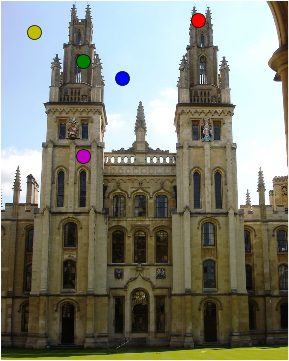
\includegraphics[width=.48\textwidth]{points1}
    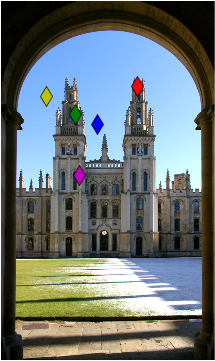
\includegraphics[width=.48\textwidth]{points2}
  \end{center}
  \caption{\emph{Left:} Certain points are selected on the original image. \emph{Right:} Points generated by the provided homography. Same colored points in the left and right image form an input and output pair.}
  \label{fig:points}
\end{figure}

\section{Compute homography between two images}

\section{Image recognition with geometric verification}

\section{Bonus}
\begin{itemize}
    \item Normalization makes the data scale invariant.
    \item One way to find this, is to compute the inverse of the homography matrix:
      \begin{eqnarray*}
        x' &= H_{1,2} x \\
        H_{1,2}^{-1} x' &= H_{1,2}^{-1} x \\
        H_{1,2}^{-1} x' &= x \\
        H_{2,1} x' &= x
      \end{eqnarray*}
\end{itemize}
\end{document}
